Este problema consiste en generar la silueta de una ciudad a partir de la representaci\'on de varios edificios que la componen.
A la entrada del algoritmo voy a tener una cantidad \textbf{N} de edificios, representados con tres valores; el comienzo, su altura y dode termina. Todos los valores son enteros positivos, en relacion a cada eje, horizontal y vertical.
A la salida voy a tener representada la silueta de la ciudad como una seguidilla de puntos que representan el contorno de los edificios que \textbf{sobresalen} del resto.
La idea esto es ocultar las partes de los edificios que quedan \textbf{dentro} de otros edificios.

\subsubsection*{Escenarios t\'ipicos}
\addcontentsline{toc}{subsubsection}{Escenarios t\'ipicos}

Las siguientes instancias son las b\'asicas a las cuales se pueden reducir todos los escenarios. La primer imagen representa a los edificios que son la entrada del algoritmo con el aditivo de los puntos marcados \footnote{Aporte realizado por un compañero del curso que lo envió a la lista de mails. Todos los créditos para \'el.} que ser\'ian la solución final. Y la segunda imagen es la ciudad representada con su silueta.

\subsubsection*{Edificio B\'asico}
\addcontentsline{toc}{subsubsection}{Edificio B\'asico}
\begin{figure}[H]
\begin{center}$
\begin{array}{cc}
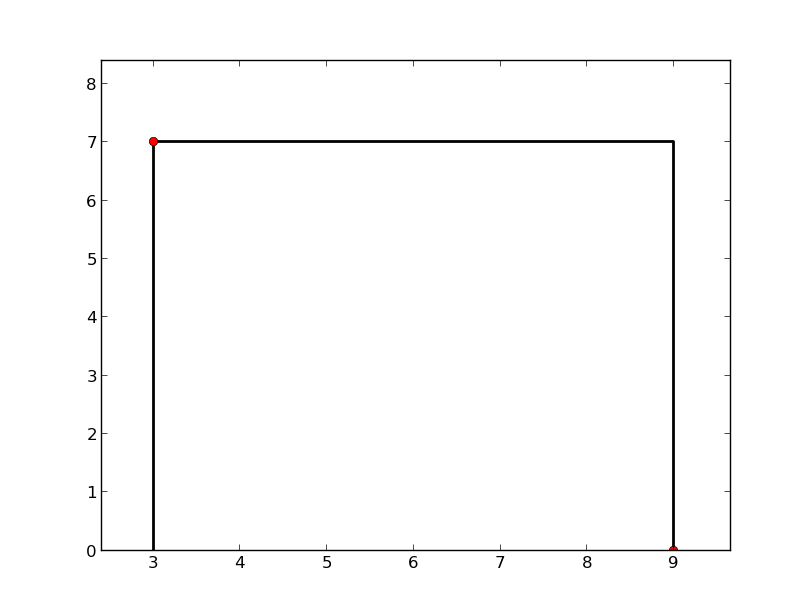
\includegraphics[scale=0.3]{./imagenes/ej2_edificio1.png}&
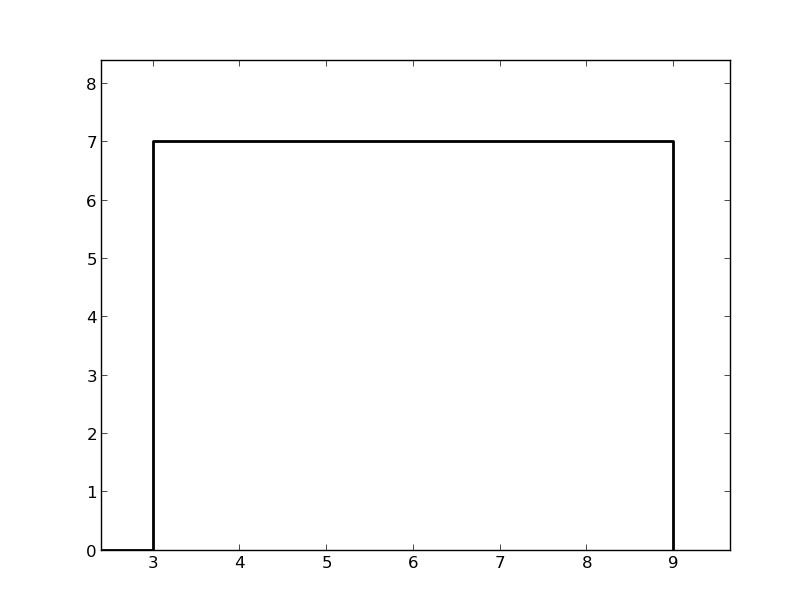
\includegraphics[scale=0.3]{./imagenes/ej2_edificio1solucion.png}
\end{array}$
\end{center}
\caption{Una ciudad con un solo edificio}
\end{figure}

\subsubsection*{Edificios Cruzados 1}
\addcontentsline{toc}{subsubsection}{Edificios Cruzados 1}
\begin{figure}[H]
\begin{center}$
\begin{array}{cc}
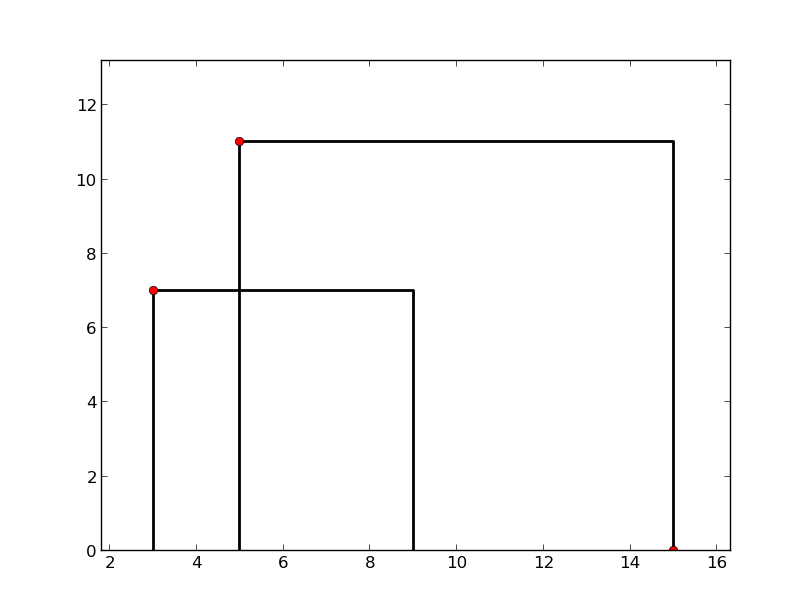
\includegraphics[scale=0.3]{./imagenes/ej2_edificio2.png}&
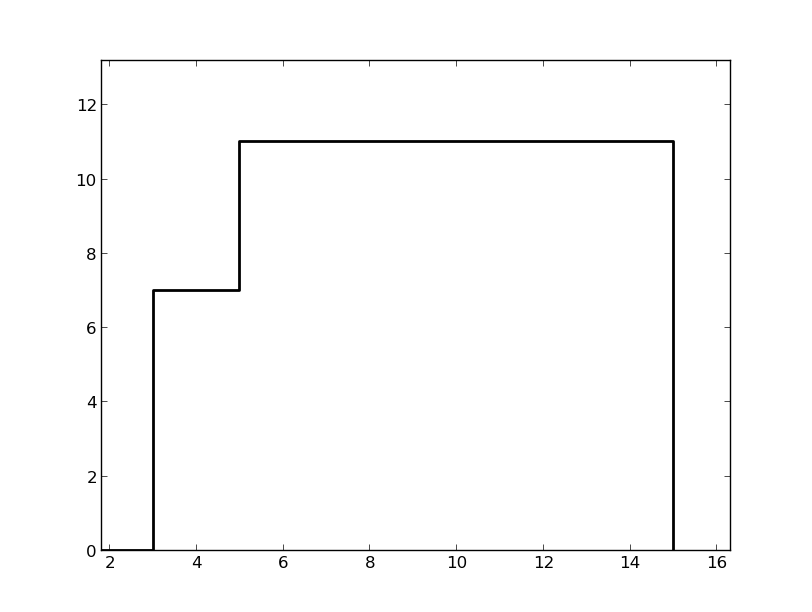
\includegraphics[scale=0.3]{./imagenes/ej2_edificio2solucion.png}
\end{array}$
\end{center}
\caption{Edificios Cruzados 1}
\end{figure}

\subsubsection*{Edificios Cruzados 2}
\addcontentsline{toc}{subsubsection}{Edificios Cruzados 2}
\begin{figure}[H]
\begin{center}$
\begin{array}{cc}
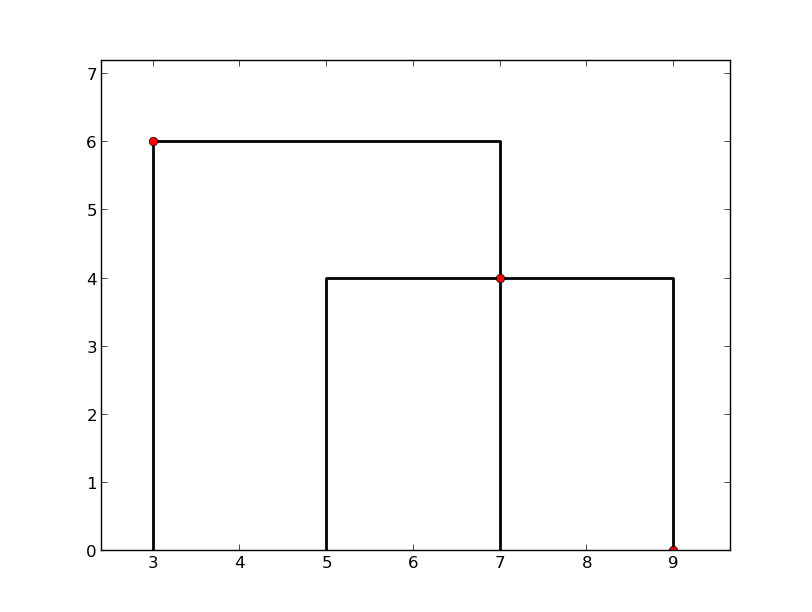
\includegraphics[scale=0.3]{./imagenes/ej2_edificio3.png}&
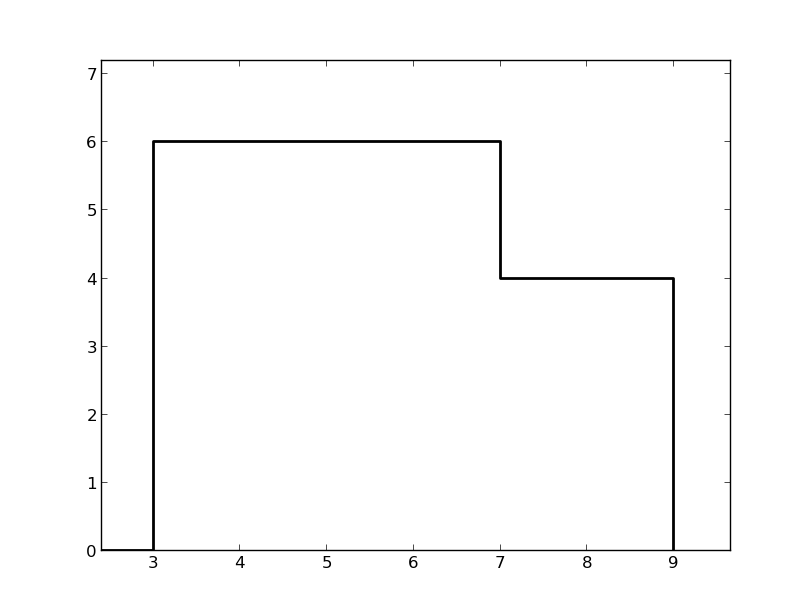
\includegraphics[scale=0.3]{./imagenes/ej2_edificio3solucion.png}
\end{array}$
\end{center}
\caption{Edificios Cruzados 2}
\end{figure}

\subsubsection*{Edificios Solapados}
\addcontentsline{toc}{subsubsection}{Edificios Solapados}
\begin{figure}[H]
\begin{center}$
\begin{array}{cc}
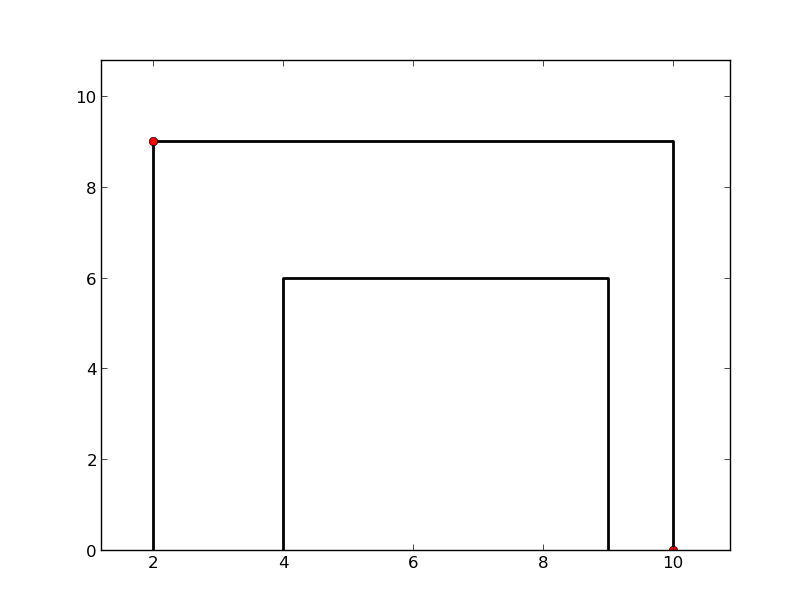
\includegraphics[scale=0.3]{./imagenes/ej2_edificio4.png}&
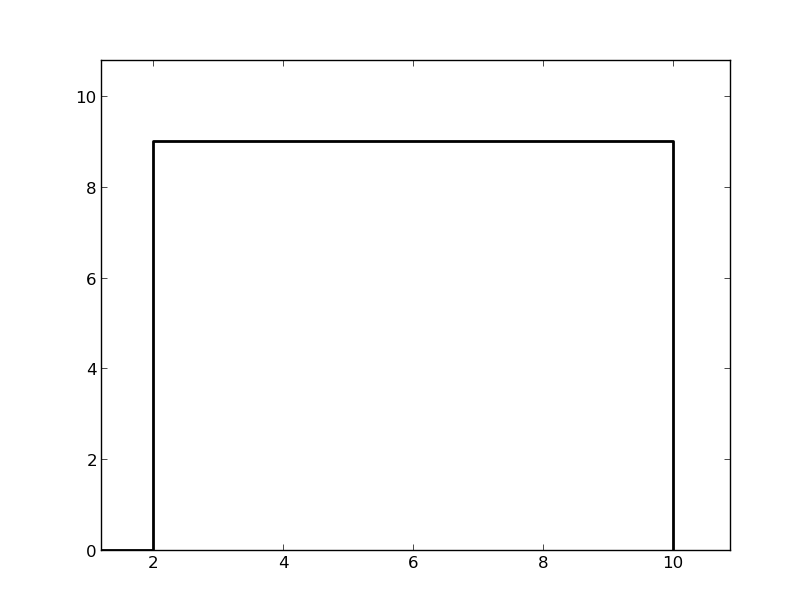
\includegraphics[scale=0.3]{./imagenes/ej2_edificio4solucion.png}
\end{array}$
\end{center}
\caption{Edificios Solapados}
\end{figure}

\subsubsection*{Edificios Contiguos}
\addcontentsline{toc}{subsubsection}{Edificios Contiguos}
\begin{figure}[H]
\begin{center}$
\begin{array}{cc}
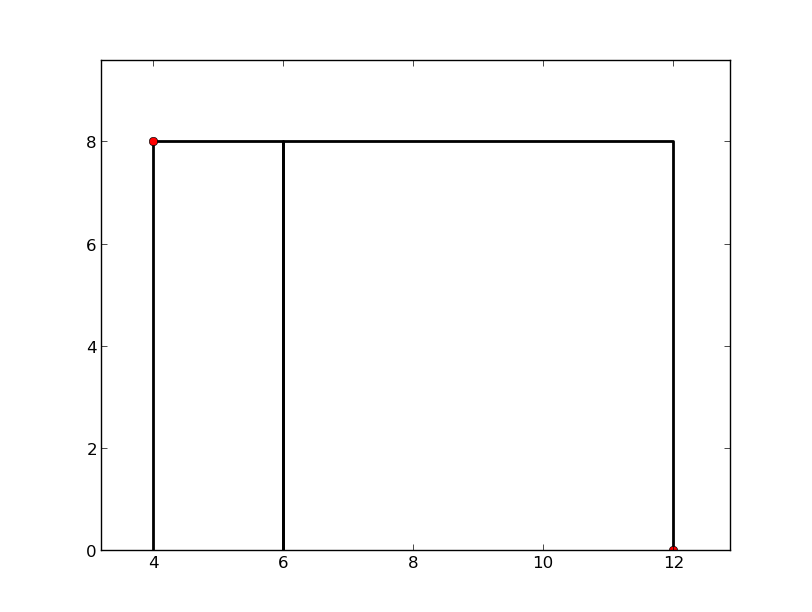
\includegraphics[scale=0.3]{./imagenes/ej2_edificio5.png}&
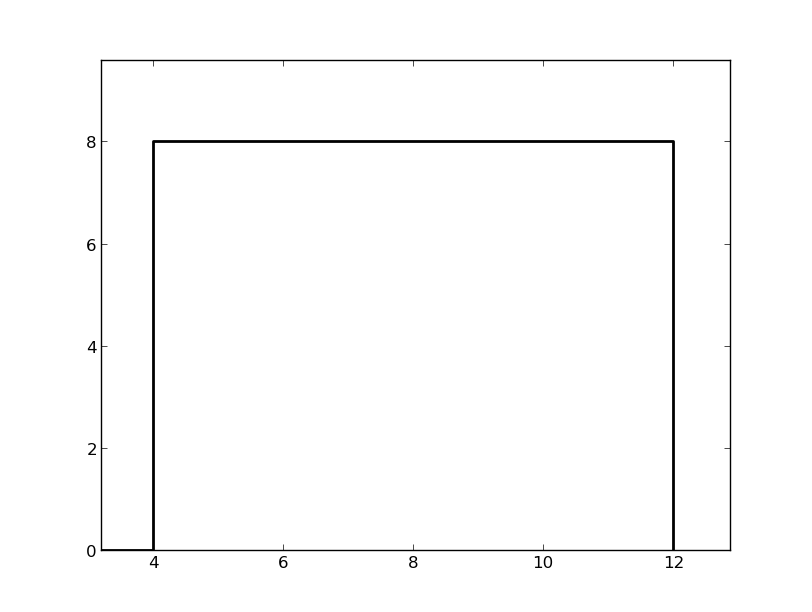
\includegraphics[scale=0.3]{./imagenes/ej2_edificio5solucion.png}
\end{array}$
\end{center}
\caption{Edificios Contiguos}
\end{figure}


\subsubsection*{Edificios Varios}
\addcontentsline{toc}{subsubsection}{Edificios Varios}
\begin{figure}[H]
\begin{center}$
\begin{array}{cc}
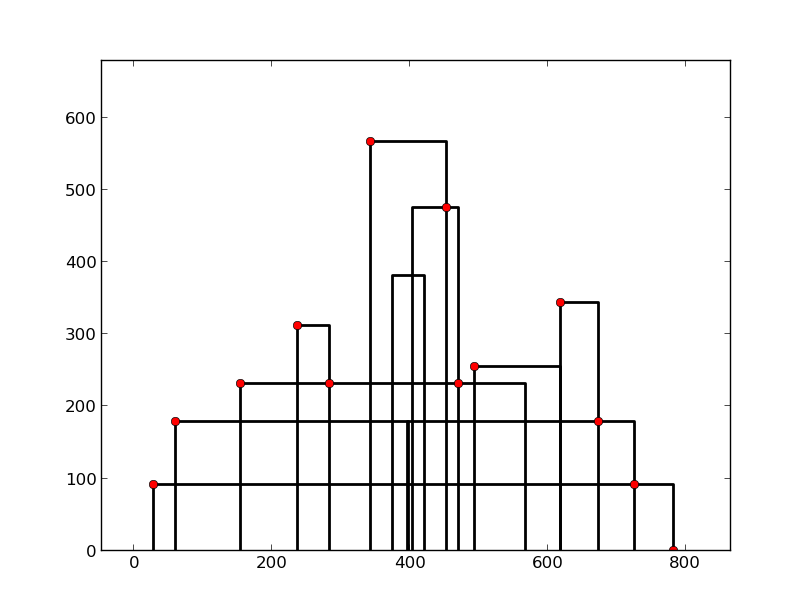
\includegraphics[scale=0.4]{./imagenes/ej2_edificio6.png}&
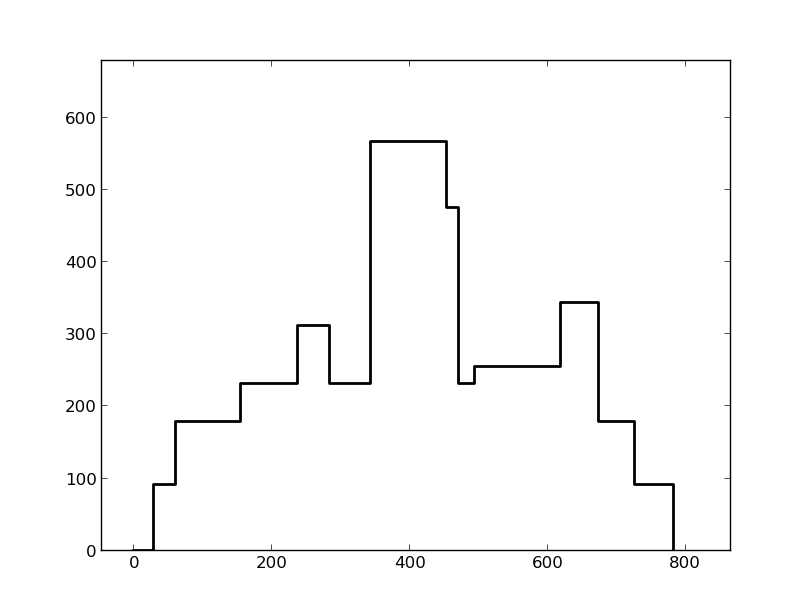
\includegraphics[scale=0.4]{./imagenes/ej2_edificio6solucion.png}
\end{array}$
\end{center}
\caption{Edificios Varios}
\end{figure}